\itemhead{3.1 例题 · 例题8（教材p.75）}{XJ-B1-C03-EX-P075-Y0639}
\label{XJ-B1-C03-EX-P075-Y0639}
{\footnotesize 湘教版教材p.75 / PDF第82页 / 3.1 例题 / 例题8}
\field{原题}{画出函数 $f(x)=|x-2|+|x+1|$ 的图象。}
\field{参考答案}{$f(x)=\begin{cases}1-2x,&x<-1,\\3,&-1\le x\le2,\\2x-1,&x>2.\end{cases}$，按两条射线与水平线段画图，转折点为 $(-1,3),(2,3)$，值域 $[3,+\infty)$。}
\begin{center}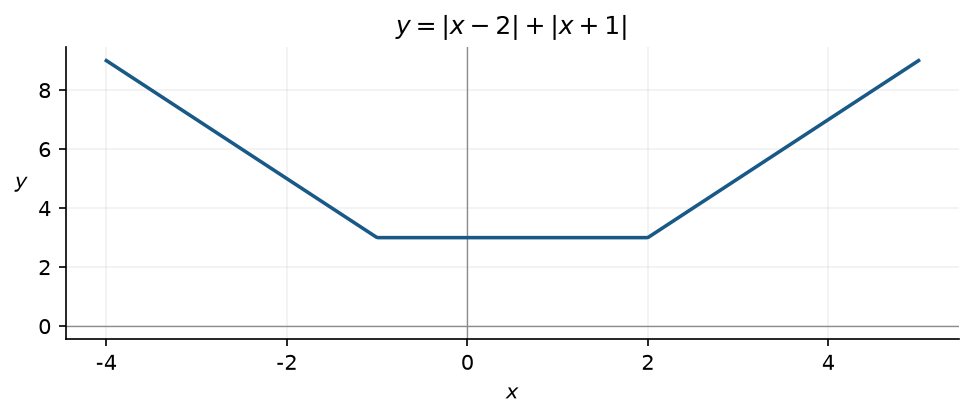
\includegraphics[width=.84\linewidth,height=.38\textheight,keepaspectratio]{figures/C03-EX075-8.png}\end{center}
{\small \field{关联知识}{F07 分段函数、绝对值及分段应用（教材帮p.86、91、92、93 / PDF95、100、101、102）；F04 函数三种表示法、图象与读数（教材帮p.85、86、93、94 / PDF94、95、102、103）}
\field{方法与易错点}{先列转折点和各段条件，再建立分段式，检查衔接、定义域与值域。 易错：跨段套公式；超额部分按全量收费；绝对值去号漏区间。}
\field{答案依据}{例题原解位置：湘教版教材p.75及题库原图；独立编写可编辑参考解答。答案册此部分主要收练习、习题，不伪造例题答案册位置。}}
